% 2007 年全国大纲卷Ⅰ理科第 19 题：四棱锥
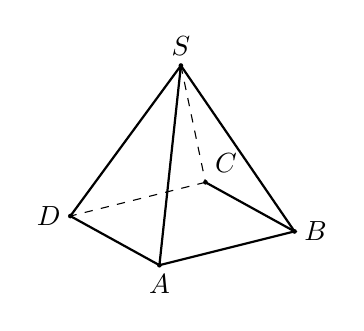
\begin{tikzpicture}[>=stealth,scale=0.78]
  \coordinate (A) at (1.8,0); \coordinate (B) at (4.0,0.55);
  \coordinate (C) at (2.55,1.35); \coordinate (D) at (0.35,0.8);
  \coordinate (S) at (2.15,3.25);
  \draw[thick] (A)--(B)--(C); \draw[dashed] (C)--(D); \draw[thick] (D)--(A);
  \draw[thick] (S)--(A) (S)--(B) (S)--(D);
  \draw[dashed] (S)--(C);
  \fill (S) circle (1.1pt) node[above] {$S$};
  \fill (A) circle (1.1pt) node[below] {$A$};
  \fill (B) circle (1.1pt) node[right] {$B$};
  \fill (C) circle (1.1pt) node[above right] {$C$};
  \fill (D) circle (1.1pt) node[left] {$D$};
\end{tikzpicture}
